% !TEX root = ../master.tex
\chapter{Design and Methodology}
\label{chap:design}
This chapter describes which research method is used to design a solution 
that answers the initial questions posed in the first chapter.
The considerations that contribute to the design of this solution are outlined 
and form the foundation for its implementation in the next chapter.

\section{Employed Methodology}
\label{sec:design:methodology}

Preceding to the practical part of this thesis, 
the method to follow along shall be laid out here.
One suitable method is the general concept of \emph{design science research}, also known as \emph{constructive research}, 
since it involves the development and evaluation of artifacts to solve domain specific problems.
It, therefore, conveys an improved practical relevance in comparison to purely descriptive research methods,
while the outcomes still create scientific knowledge
\autocite[][p.~v]{dresh2015designresearch}.
The conducted research must design an artifact, such as a construct, model or method, that solves a relevant problem in a specific field, which is evaluated regarding its utility, quality, and efficacy.
The performed research should be based on rigorous scientific methods and contribute to the current theoretical body of knowledge.
The conducted design process must take into account the practical environment it is executed in and use the available resources.
A conclusion of the project for both technology-oriented as well as management-oriented audiences should be presented in the end
\autocite[][p.~70]{dresh2015designresearch}.

\begin{figure}[hbt]
	\centering
	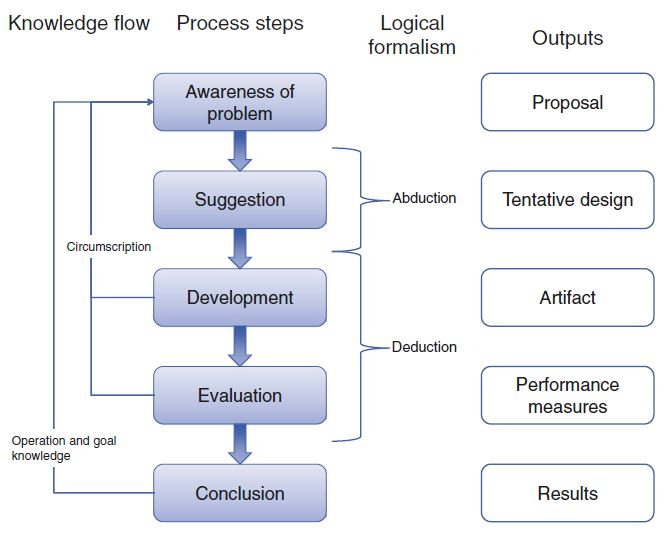
\includegraphics[width=0.8\textwidth, keepaspectratio]{resources/designscienceresearchoutputs.jpg}
	\caption[Process steps and outputs of design science research]{\label{fig:design:designscience} Process steps and outputs of design science research. Reprinted from \textcite[][p.~83]{dresh2015designresearch}}
\end{figure}

Figure \ref{fig:design:designscience} displays the steps that are found in the process of design science research. 
Those are the steps that guide the execution of this thesis.
The awareness and relevance of the given problem have already been given in section \vref{sec:into:context}.
Looking back to the original research questions (see section \vref{sec:intro:goals}) two focuses have been identified for this thesis:

\begin{itemize}
    \item Which computer vision techniques can be used to detect persons and objects within an elevator car and in front of the lift and estimate their spacial volume?
    \item How can the information acquired by a system that uses such methods constitute to the optimization of algorithms that control the movement plan for elevators?
\end{itemize}


To answer the two questions, the conducted research is therefore twofold.
The first part involves the design and experimental implementation of a system to gather passengers volume data in elevators.
The second part deals with the integration of this information into a scheduling algorithm.
Outlined below are the steps that are taken to
suggest a tentative design for each, develop the artifacts and evaluate them.

For the  design and implementation of a vision system to gather volume data of passengers,
the following steps are performed:

\begin{enumerate}
    \item Find a typical or actual elevator control system architecture and define the positions to integrate the necessary components for a vision system into it.
    \item Define the exact type and structure of the information that the vision system should be able to detect.
    \item Find an algorithmic approach to  passenger detection and volume estimation that is suitable to generate the required data.
    \item Match the approach with a possible hardware setup to perform tests with it.
    \item Test the proposed detection system in a real-world experiment that includes  exemplary footage from within a cabin.
    \item Evaluate the results of the test for the functionality and effectiveness of the employed system.
\end{enumerate}

For the integration of the passenger data into an existing scheduling algorithm the following steps are performed:

\begin{enumerate}
    \item Define a suitable elevator configuration that, could possibly benefit from the information that the vision system can provide. 
    Find a typical or actual control algorithm that is used for such a configuration.
    \item Adapt the scheduling algorithm to use the additional information.
    \item Compare the two versions of the algorithm in order to determine their effectiveness regarding a suitable metric.
    A simulation is used to perform this comparison.
\end{enumerate}

%\begin{figure}[hbt]
%	\centering
%	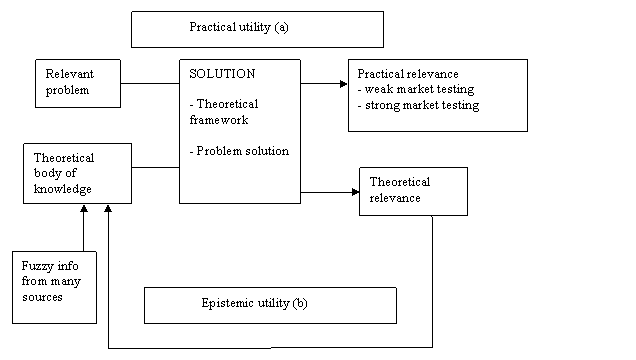
\includegraphics[width=1.0\textwidth, keepaspectratio]{resources/Rasvan_constructive_research_diagram}
%	\caption{\label{fig:design:constructiveresearch} Elements of constructive research. Source:
%	\url{https://en.wikipedia.org/wiki/File:Rasvan_constructive_research_diagram.gif}}
%\end{figure}
 
\section{Visual System}
The section ahead describes the design of a camera-based visual system that is able to capture the volume of passengers that are using an elevator system. 
in order to design this system, the approach described in the previous section is followed.
First, the integration into a typical elevator system is described, 
then the detection capabilities of the system are specified.
Building on that, an approach to the volume detection is constructed.
In the next chapter, an exemplary implementation of this approach is created.

The \emph{Otis Elevator Company} hold patents, which describe a similar but more extensive elevator control system \autocite[][]{lin2011control} \autocite[][]{xang2016trafficlist}.
The two patents describe systems with a much broader scope.
They focus on tracking individual passengers over their whole journey and use this data for scheduling, door control, and security \autocite[][]{lin2011control}. 
By generating a \enquote{traffic list} from objects recognized in a depth map of they extended this concept also to volume tracking \autocite[][]{xang2016trafficlist}.

\subsection{Proposal for Integration into Elevator Control System Architecture}

There are two places in an elevator system, where the addition of a camera system can create information about passengers: inside the cabin and in front of the lift in the main or floor halls.
Cameras inside the cabin could determine, if passengers are currently occupying the space in it and if additional large cargo objects are inside.
Cameras in the hall on each floor can observe passengers, that are about to perform a hall call.
However since this paper explores the possibilities of volume detection, 
the information gathered inside the cabin is focused.

In the context of an elevator system, 
the cameras inside the cabin are, 
combined with a processing system, 
are just an additional cabin sensor.
Therefore the system can be integrated into the electronics of the elevator cabin
and is attached to the elevator controller, 
which can interact with it to make use of the gathered data.
If the visual system should be integrated into a multi-cabin system, 
the elevator controller can forward the information from the visual system to the group controller.
Figure \ref{fig:design:systemintegration} visualizes the proposed integration.

\begin{figure}[htb]
    \centering
    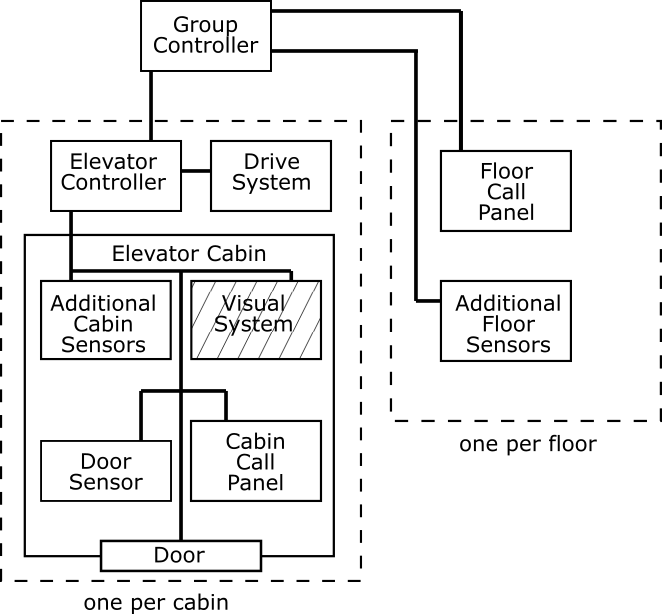
\includegraphics[width=0.8\textwidth, keepaspectratio]{systemcomponets_with_visual}
    \caption[Elevator system extended with visual system]{Elevator system extended with visual system. Addition to figure \ref{fig:sota:systemcomponents}}
    \label{fig:design:systemintegration}
\end{figure}

\subsection{Output Data Definition}

It is the purpose of the visual system to provide information about the volume of passengers and cargo objects.
Therefore it should generate the following pieces of data: 

\begin{itemize}
    \item The total number of passengers and cargo objects inside the cabin.
    \item The approximate volume of each passenger or cargo object.
    \item The approximate dimensions of each passenger or cargo object.
\end{itemize}

The system should operate in near real time,
meaning the output data should match the current situation inside the cabin.
Only a short time may be taken up for processing the image data.
Otherwise, the situation inside the cabin could change significantly during the processing time, which would make the information gathered by the system less meaningful.
In an elevator, this change can happen in seconds, for example when passengers are entering and leaving the cabin.

\subsection{Detection Technique}
\label{sec:design:detection}

The technique to generate the data that which has been defined above,
is centered around the reconstruction of the volume that is occupied by the passengers and objects inside the cabin.
Figure \ref{fig:design:volumedetection} displays the general concept of this technique.
The left side of the figure exhibits the data that is input for the system, 
the right side shows, which steps are taken to process this data inside the system.
First the video capture from the cameras inside the cabin is read, which gets processed and combined with the position and calibration data of the cameras in order to create a reconstruction of the volume inside the cabin.
This volume representation is then used to take measurements of the passengers and objects inside the cabin.
The next paragraphs describe each of these steps in more detail.

\begin{figure}[hptb]
    \centering
    \tikzset{
        box/.style = {
            draw, 
            rectangle, 
            rounded corners, 
            minimum height = 2.5em, 
            minimum width = 2.5em, 
            text width=10em, 
            text centered,
            thick
        },
        to/.style = {
            ->,
            >=stealth',
            shorten >=1pt,
            thick,
            font=\sffamily\footnotesize
        }
    }
    \begin{tikzpicture}[auto, node distance=3em]
        \node (cap) [box] {Video Capture};
        \node (pre) [box, right = of cap] {Preprocessing};
        \node (mask) [box, below = of pre] {Foreground Masking};
        \node (space) [box, below = of mask] {Volume Reconstruction};
        \node (calib) [box, left = of space] {Camera Calibration Data};
        \node (blob) [box, below = of space] {3D Blob Detection};
        \node (meas) [box, below = of blob] {Blob Measurement};
        \node (class) [box, below = of meas] {Blob Classification};
        \draw [to] (cap) -- (pre);
        \draw [to] (pre) -- (mask);
        \draw [to] (mask) -- (space);
        \draw [to] (space) -- (blob);
        \draw [to] (calib) -- (space);
        \draw [to] (blob) -- (meas);
        \draw [to] (meas) -- (class);
    \end{tikzpicture}
    \caption{Volume detection technique}
    \label{fig:design:volumedetection}
\end{figure}

\subsubsection{Video Capture}
Inside the cabin, multiple cameras are mounted.
The cameras are positioned on the walls of the cabin, such that they observe the center of it.
On each wall, one can be mounted.
Where it is not possible to place the camera on the wall, for example on the side of the doors,
it is also possible to position the camera in the ceiling corner.
This way the space in the cabin is viewed from multiple angles, 
which enables ever position in the cabin to be observed by cameras. 
Using cameras of the same model and optic configuration makes the implementation easier.
The cameras are connected to the processing unit of the visual system and provide a lifestream of image frames to it.

\subsubsection{Preprocessing}
As the first active step, the images of all the cameras 
are read into the memory of the system as \ac{2D} color images 
with the native resolution of the cameras.
In order to decrease the computation power needed for the next steps, 
it is possible to \emph{scale them down} to a smaller size.
Furthermore, the camera images typically contain noise, 
which can be countered by applying a \emph{Gaussian blur} filter so it.
The convolution kernel $ G $ shown in figure \ref{fig:sota:kernels} is a candidate,
but also Gaussian kernels of dimension $ 5 \times 5 $ can be used.

\subsubsection{Foreground Masking}
To find out where passengers and objects are visible in each frame from each camera the next step is to find a foreground mask for each of the images.
Since the cameras are static and do not change their position or angle in the cabin,
each camera always films the same section of the elevator.
The perceived background therefor is static except for changes in lighting.
Those can occur when the cabin doors are opened or passengers block the lamps in the cabin.
In contrast to the background, the passengers in the cabin move over time.
The static background with moving passengers allows the method of \emph{background subtraction} to be used.
Either static or dynamic techniques can be used, 
but the dynamic approach of the \ac{MOG} is favorable, 
since it can react to changes in lighting.

The resulting foreground masks might be noisy and can have pixel-sized artifacts.
These originate from noise present in the processed image and small changes between two frames in locations, where actually no passenger is present. 
In order to remove this noise in the binary foreground mask, the morphological \emph{OPEN} operation is used. 
It is a sequential application of the \emph{ERRODE} and \emph{DILATE}, which first removes all edge pixels and then extends the remaining edges again.
This way, single active pixels are deleted, while other structures are preserved.
After this, the \emph{DILATE} operation is applied again to close potential holes in the masks.

\subsubsection{Camera Calibration}
In this step, the internal and external parameters for all cameras are gathered.
Since the camera settings are not altered during the operation of the system, these parameters only need to be determined once and can then be reused.
The following parameters must be obtained for each camera, which is also explained in figure \ref{fig:sota:camcalib}:
\begin{itemize}
    \item The internal camera matrix $ A $, which includes the focal length and the point of the image center. They can be obtained from calibration footage that features an identifiable object of known geometry, such as a chess board.
    \item The external rotation matrix $ R $ and the translation vector $ t $, which can be obtained by measuring the position and viewing direction of the camera.
    \item The internal distortion coefficients of the camera, which also can be obtained from calibration footage.
\end{itemize}

Additionally to the camera parameters, the dimensions of the elevator cabin need to be known to be later able to convert pixel units into world units of meter.
The parameters obtained in this step are used in the next step to guide the volume reconstruction.

\subsubsection{Volume Reconstruction}

From the camera calibration and position data and the foreground mask of each perspective, 
it is possible to reconstruct the volumetric data of the interior of the cabin.
The technique of \emph{volume intersection} is used for this.
Since the purpose of this system does not require a photo-realistic, the simple voxel-based method can be used.
It would be possible to reconstruct the full geometry and color of the room using a point matching algorithm or the more advanced space carving. 
However, it is not necessary to reach such a level of detail for the purpose of this system.

In the volume intersection technique, first, the whole volume of the elevator is described as a \ac{3D} image of $ X \times Y \times Z $ voxels.
The number of voxels is chosen rather low, in total between 10,000 and 100,000.
If a larger amount is chosen, results with higher accuracy could be obtained at the expense of processing power.
The voxels describe an evenly distributed cube grid, that fills the whole elevator cabin.
In order to perform the volume reconstruction,
the position of every voxel is projected into the viewport of each camera by applying the formula given in figure \ref{fig:sota:camcalib} to it with the parameters obtained from the camera calibration in the step before. 
This projection also needs to take the transformation from world coordinates in meter into pixel coordinates in the camera into account.
Now a \ac{3D} binary image $ F_{vol} \in \{0, 1\}^{X \times Y \times Z} $ is created, by checking for every voxel if it lies within the viewport of each camera and is projected to a foreground pixel in it.
If this is the case for all cameras, the voxel is considered to be part of an occupied volume and hence marked as 1, otherwise as 0.

\subsubsection{3D Blob Detection}

The volume intersection in the previous step yielded a \ac{3D} binary image \\
$ F_{vol} \in \{0, 1\}^{X \times Y \times Z} $, where voxels marked with $ 1 $ indicate the presence of an object or passenger at the position of the volume element.
Where ever a passenger or object takes up space in the \ac{3D} image, a \ac{3D} \emph{binary blob} is present, which is a collection of spacial coherent voxels that are positively labeled.
In order to find distinct entities in that image, the \emph{connected component labeling} method can be used.
Initially introduced for \ac{2D} images, it is possible to extend 
the common label-propagation and label-equivalence algorithms to work on a binary image of higher dimensions
\autocite[][p.~39]{he2017connected}.
Since $ X, Y, Z $ have been chosen to be of low resolution, it appears appropriate to use a label-propagation approach.

In a simplified version of this approach, the \ac{3D} image is scanned in a raster, 
and each encountered voxel, which is labeled as 1 in $ F_{vol} $ and has not yet been labeled by the connected component algorithm, it assigned a new unique label.
Furthermore, all neighboring voxels, which are labeled as 1 in $ F_{vol} $, are also labeled with this label.
When a voxel is encountered, which is already labeled, this label is also propagated to its neighbors that are labeled as 1 in $ F_{vol} $. 
The basics of this approach work exactly like in two dimensions, however, the definition of neighboring voxels is altered to match three dimensions. 
In general, all 26 voxels in the cube around a voxel are considered neighbors.
It is also possible to only consider the 6 voxels, that share a face with the center voxel.

The described algorithm performs a mapping $ \{0, 1\}^{X \times Y \times Z} \rightarrow \mathbb{N}^{X \times Y \times Z} $, where the voxel values of the output represent the unique label of the blob they belong to, or 0 in case that the voxel does not belong to any blob.
Has a complexity of $ \mathcal{O}(X Y Z) $ and operates without additional memory. 
The algorithm can be improved by performing the label-propagation along the surface of the \ac{3D} blobs.

\subsubsection{Blob Measurement}

The previous step yielded a \ac{3D} image $ F_{blobs} $ consisting of labeled binary blobs.
For each blob, the volume and its length in the X, Y and Z axis are calculated.
The volume is calculated by summing up the volume of the voxels, which make up the blob.
Even when no concrete volume for each voxel is known, this volume is still proportional to the total volume of the containing image $ F_{vol} $.
The length in a particular axis can be found  by calculating the distance of the two most extreme voxels in that axis that belong to the blob.
Figure \ref{fig:design:blobmeasurement} describes the calculations for this measurements for a blob with label $ l $.

\begin{figure}[h!]
\centering{
$$ P_l = \{ (x, y, z) | F_{blobs}(x, y, z) = l\} $$
$$ \Delta{}X_{l} = max(\{ x | (x, y, z) \in P_l \}) - min(\{ x | (x, y, z) \in P_l \}) $$
$$ \Delta{}Y_{l} = max(\{ y | (x, y, z) \in P_l \}) - min(\{ y | (x, y, z) \in P_l \}) $$
$$ \Delta{}Z_{l} = max(\{ z | (x, y, z) \in P_l \}) - min(\{ z | (x, y, z) \in P_l \}) $$
$$ V_{l} = ||P_l|| \cdot V_{voxel} = \sum\limits_{P_l}^{}V_{voxel} $$
}
\caption{Calculation of 3D blob measurements}
\label{fig:design:blobmeasurement}
\end{figure}

\newpage

\subsubsection{Blob classification}
With the aid of the previously generated measurements, each blob can be classified to find out whether it reassembles a passenger, a group of passengers, or a large cargo object.
Blobs with a volume smaller than a specific threshold $ T_{min} $ are probably erroneous artifacts and can easily be ignored.
If the volume is human like and the proportions of the blob are higher then wide, it can be classified as a human. 
If the volume is larger than a threshold $ T_{max} $ or if the blob has a greater width than height, it can be either classified as a large object, or as a group of passengers.

An alternative to this static approach would be to apply machine learning algorithms to find out the classification of a blob.
For this, a pre-classified learning data set needs to be available, which might not be feasible.

\subsection{Test Arrangement and Validation Strategy}
\label{sec:design:visualtest}
To show the general feasibility of the approach described above, 
a real live test is performed.
For this test, an exemplary office elevator is used.
Inside it, multiple cameras are mounted at the walls, 
all viewing the center of the cabin.
The cameras do not capture a live stream that is processed but record a video for later processing.
Four cameras are used in the test configuration.
One mounted to the center of each wall of the elevator, in a height of 150~cm.
These cameras are therefore positioned at a right angle towards each other.
An additional camera is mounted over the entry door within the elevator, also facing the center of the elevator.

During the performance of the test, there are multiple scenarios
of passengers residing in the cabin:
\begin{itemize}
    \item Empty cabin
    \item Single passenger in multiple positions in the cabin
    \item Multiple passengers in multiple positions in the cabin
    \item Single passenger with a large cargo object in the cabin
    \item Multiple passengers with a large cargo object in the cabin
\end{itemize}
In the test, each of those scenarios is conducted for about a minute or less.

A typical approach to evaluate the performance of a 
quantitative algorithm in computer vision is to compare it against the \emph{ground truth} present in the observed scene.
The ground truth is a description of the scene in the same format which the algorithm produces, however it is generated by inspection of the original scene by a human.
If the description consists of data for which an order exists, this order can be used for evaluation of the capability of the system.
In general, however, the data that is compared might be arbitrarily complex and therefore it is not always possible to perform the comparison quantitatively. Rather a human has to decide, how \enquote{good} the produced results are.


\section{Scheduling Algorithm}
\label{sec:design:schedulingalgorithm}
This section describes the design of a scheduling strategy, 
which makes use of the information provided by the visual system designed above.
The strategy is tailored to meet the needs of a building, in which passengers and cargo objects are sharing a lift.
The strategy is then compared against conventional scheduling algorithms by designing a simulation of an elevator system that runs those algorithms.
This section follows the line of action defined in section \ref{sec:design:methodology}.
In the next chapter, the results of this simulation are explored.

\subsection{Suitable Elevator Configuration}
Since the camera system is suitable to detect passengers as well as cargo objects,
it seems reasonable to apply the passenger information 
to a scheduling algorithm of an elevator system which conveys both of them.
This holds the opportunity to have a bigger impact on the performance of the system, 
in contrast to applying it to a passenger-only lift.

When looking back at the categorization of elevators, cargo lifts meet this specification.
Typically an office building has one or multiple cargo lifts depending on its size,
but grouping them is uncommon \autocite[][p.~167]{barney2016handbook}.
A weight capacity of at least 1,600 kg is typical \autocite[][p.~167]{barney2016handbook},
but also capacities of 5,000 kg are possible \autocite[][]{kone2017overview}.
Typical application areas for cargo lifts are hospitals, where patients and beds are moved,
auxiliary lifts in office buildings and multi-storey industrial buildings.
The typical control algorithm is collective control or sequential control \autocite[][pp.~238,~244]{barney2016handbook}.
For this comparison, the sequential control and collective control will be taken as a baseline.

\subsection{Adaption of Scheduling Algorithm}
The proposed visual system is able to detect, whether a passenger or a large object is present in the cabin.
This information holds the possibility to be used in an appropriate elevator scheduling algorithm.
Therefore a new control strategy is proposed here, which will be called \emph{adaptive control} in the following. 
The strategy is a combination of collective control and sequential control.
It follows these simple rules:

\begin{itemize}
    \item When no cargo item is present in the cabin, the elevator is operated in collective mode and picks up and delivers passengers according to the collective control strategy.
    \item When there is a cargo item present in the cabin, deliver it directly to its destination car call, regardless of other car calls and hall calls.
\end{itemize}

Since those rules make use of the information about the destination floor of the cargo object, the necessity to associate the cargo item to its car call within the system is implied.
This association can be determined from the combination of the video data and car call data.
When the cargo object is first detected, one of the next car calls made must be from the object or the passenger escorting it.

\subsection{Preparation for Simulation and Validation Strategy}

\subsubsection{Scheduling Algorithms}
\label{sec:design:schedulingalgorithms}

As discussed before the introduced \emph{adaptive control strategy} is evaluated using a simulation of an elevator system. 
It is compared against the \emph{sequential control strategy} and the \emph{collective control strategy}.
In order to guide the implementation of the simulation, the concrete actions that these three strategies take to move an elevator are laid out in the following.

The \textbf{sequential control strategy} delivers one passenger at a time and serves hall calls sequentially. 
Its behavior can be described with the following actions:
\begin{enumerate}[noitemsep]
    \item Update the queue of hall calls by appending all active hall calls that are not yet in the queue.
    \item If there is an active car call:
    \begin{enumerate}[noitemsep]
        \item Move to is respective floor.
        \item Open the doors.
        \item Unload the passenger. 
        \item Close the doors. 
        \item Clear the car call.
    \end{enumerate}
    \item Otherwise, if there is an hall call in the queue:
    \begin{enumerate}[noitemsep]
        \item Move to the floor of the first hall call in the queue. 
        \item Open the doors.
        \item Load one passenger into the lift. 
        \item Delete the hall call from the queue.
        \item Update the car call to be the destination floor of the passenger.
    \end{enumerate}
\end{enumerate}

The \textbf{non-directional collective control strategy} collects and drops off passengers along the way while serving the hall and car calls.
Its behavior can be described with the following actions:
\begin{enumerate}[noitemsep]
    \item Let the car calls be all the destinations of all passengers present in the lift.
    \item Let the hall calls be all the unique floors where passengers wait for the elevator
    \item If the car calls contain the current floor:
    \begin{enumerate}[noitemsep]
        \item Open the doors.
        \item Unload the passengers for this floor.
    \end{enumerate}
    \item Otherwise, if the hall calls contain the current floor:
    \begin{enumerate}[noitemsep]
        \item Open the doors.
        \item Load all passengers on the floor into the lift, which fit in it.
    \end{enumerate}
    \item Otherwise, if there is another car call or hall call in the current direction of travel:
    \begin{enumerate}[noitemsep]
        \item Close the doors.
        \item Move to the closest car call or hall call in the direction of travel.
    \end{enumerate}
    \item Otherwise reverse the current direction of travel.
\end{enumerate}

The \textbf{adaptive control strategy} introduced before makes a decision based on whether a cargo object is currently located inside the cabin.
Its behavior can be described with the following actions:
\begin{enumerate}[noitemsep]
    \item If there is a cargo object in the elevator:
    \begin{enumerate}[noitemsep]
        \item Close the doors.
        \item Move to its destination floor.
        \item Open the doors.
        \item Unload the cargo object and other passengers with this destination.
        \item Reset the current travel direction.
    \end{enumerate}
    \item Otherwise, follow the collective control strategy.
\end{enumerate}

\subsubsection{Simulation Parameters}

\begin{table}[]
\centering
\begin{tabular}{lrl}
\textbf{Description} \hspace{4cm}   & \textbf{Value}   & \textbf{Unit}   \\
\hline
\multicolumn{3}{l}{\textbf{Building data}} \\
Number of floors & 8 &        \\
Interfloor distances & 3.5 & $m$\\
%& & \\
\hline
\multicolumn{3}{l}{\textbf{Lift data}}     \\
Number of lifts & 1 & \\
Rated weight load & 5000 & $kg$\\
Rated passenger capacity & 65 & \\
Rated Speed & 1.6 & $ms^{-1}$ \\
Door opening time & 1.5 & $s$\\
Door closing time & 1.5 & $s$\\
Flight time single floor & 8 & $s$\\
%& & \\
\hline
\multicolumn{3}{l}{\textbf{Passenger Data}}\\
Arrival rates for floors & $ (f, t) \mapsto \frac{7}{300} $ & $ \mathbb{N} \times s \rightarrow s^{-1}$\\
Weight and volume distribution & see table \ref{tab:design:trafficitemprototypes} & $kg \times m \times m \times m \rightarrow \mathbb{R}$\\
%Volume distribution & see below  & $m \times m \times m \rightarrow \mathbb{R} $\\
Transfer time into / out of car & 2 & $s$\\
Floor bias & unbiased & $ \mathbb{N} \times \mathbb{N} \rightarrow \mathbb{R} $ \\
%& & \\
\hline
\multicolumn{3}{l}{\textbf{Cargo Data}}\\
Arrival rates for floors & $ (f, t) \mapsto \frac{2}{300} $ & $\mathbb{N} \times s \rightarrow s^{-1}$\\
Weight and volume distribution & see table \ref{tab:design:trafficitemprototypes} & $kg \times m \times m \times m \rightarrow \mathbb{R}$\\
%Volume distribution & see below  & $m \times m \times m \rightarrow \mathbb{R} $\\
Transfer time into / out of car & 5 & $s$\\
Floor bias & unbiased & $ \mathbb{N} \times \mathbb{N} \rightarrow \mathbb{R} $ \\
%& & \\
\hline
\multicolumn{3}{l}{\textbf{Simulation Parameters}}\\
Simulation Period & 1 & $h$\\
Time slice & 0.1 & $s$\\
Number of simulations & 1000 & \\
\end{tabular}
\caption{\label{tab:design:simulationconfig} General configuration for the comparative simulation}
\end{table}

\begingroup
\renewcommand*{\arraystretch}{1.0}
\begin{table}[htb]
\centering
\resizebox{\textwidth}{!}{%
\begin{tabular}{lrrrr}
\textbf{Type}               & \textbf{Width / cm} & \textbf{Length / cm} & \textbf{Height / cm} & \textbf{Weight / kg} \\
\hline
\multirow{4}{*}{Passenger}  & 50                  & 25                   & 160                  & 60                   \\
                            & 50                  & 25                   & 174                  & 65                   \\
                            & 50                  & 25                   & 180                  & 80                   \\
                            & 70                  & 30                   & 190                  & 110                  \\
\hline
\multirow{5}{*}{Cargo Item} & 250                 & 150                  & 150                  & 1000                 \\
                            & 250                 & 150                  & 150                  & 2000                 \\
                            & 250                 & 150                  & 150                  & 3000                 \\
                            & 250                 & 150                  & 150                  & 4000                 \\
                            & 250                 & 150                  & 150                  & 4900                
\end{tabular}%
}
\caption{\label{tab:design:trafficitemprototypes} Prototypes for traffic items in the simulation, chosen at equal likelihood}
\end{table}
\endgroup

In the section beforehand, the building type that acts as a base for the simulation has been described:
a single elevator configuration, shared by passengers and cargo items.
\textcite[][p.~347]{barney2016handbook} described, which parameters need to be determined in order to run a simulation. 
Table \ref{tab:design:simulationconfig} gives an overview of the parameters that were chosen for this simulation.
Some of the values are taken from elevators manufactured by KONE \autocite[][]{kone2017overview}, 
other values are taken from \textcite[][p.~349]{barney2016handbook}.
Especially the lift parameters are based on the sources.
In paragraphs ahead, the other parameters are discussed more thoroughly.

Table \ref{tab:design:simulationconfig} features two sections, that describe passenger data and cargo data.
The elevator can convey both, passengers and cargo objects.
Therefore, in the simulation they are both considered to be \emph{traffic items}.
Even though, not all cargo objects can move on their own, and need to be carried by a passenger,
for the purpose of this simulation, they are considered to behave identical as passengers.
In general, traffic items arrive at a certain time on a certain floor and have a defined destination floor.
The only aspect in which they differ is their arrival rate, in that more passengers than cargo objects arrive, and their physical properties.

The simulation is performed using discrete events.
Therefore a discrete, strictly increasing integer clock is used to mark the timing of events.
Each of these discrete steps is called a \emph{tick}.
The duration of such a tick is determined by the \emph{time slice} parameter.

The \emph{arrival rates} of passengers and cargo objects is chosen constant over the who time, 
which means that at any point in the simulation the chance that a given amount (0, 1, 2, ...) of traffic items arrives is fixed.
Furthermore, the arrival rate on each floor is assumed to be the same.
This behavior can be modeled with a Poisson distribution
$$ A(k) = e^{-\lambda}\frac{\lambda^k}{k!} $$
where $ A(k) $ describes the likelihood of a specific number of traffic items arriving within a time slice (duration of a tick) in the whole building.
The parameter $ \lambda $ is chosen to be the multiple of the time slice and the arrival rate.
This constant arrival model simplifies the simulation and effectively simulates an \emph{inter-floor traffic pattern}.
It would also be possible to model an up-peak or down-peak traffic pattern, however, this would make the modeling more complex.

The \emph{weight and volume distribution} for both types of traffic items is given by choosing from predefined \emph{prototypes} (or stereotypes).
Every passenger or cargo object in the simulation has the same weight and volume properties as one of the prototypes.
Table \ref{tab:design:trafficitemprototypes} lists the prototypes that are defined for this simulation.
A passenger in the simulation is created from any of the passenger prototypes with the likelihood of $ \frac{1}{4} $, a cargo item from any of the cargo item prototypes with a likelihood of $ \frac{1}{4} $.
Choosing from prototypes rather than a continuous distribution helps to simplify the simulation implementation.

The \emph{floor bias} for both types of traffic items is \emph{unbiased}. 
There is no precedence in arrival and destination floor, every journey appears with the same likelihood.
However, a journey where arrival and destination floor are equal, can not occur.
The probability of any given trip to be occur, is described as a probability function
$$ b(f_{arrival}, f_{destination}) =
    \begin{cases} 
      \frac{1}{N^2 - N} & f_{arrival} \neq f_{destination} \\
      0 & else
   \end{cases}
$$
where $ N $ is the number of floors present in a building, $ f_{arrival} $ and  $ f_{destination} $ are an integer number between 0 and $ N - 1$, which describe the arrival and destination floor number.

\subsubsection{Simulation Measurements}
To evaluate the simulations, several measurements are taken to compare the scheduling algorithms.
For the each of the measures the minimum, maximum, average and standard deviation $ \sigma{} $ values are calculated over all the simulation runs of each scheduling algorithm.  
The following measurements shall be taken:
\begin{samepage}
\begin{itemize}[noitemsep]
    \item Total passenger in the simulation
    \item Total cargo objects in the simulation
    \item Stops of the lift
    \item Delivered to their destination
    \item Cargo items delivered to their destination
    \item Waiting time
    \item Ride time
    %\item Maximum, minimum and average total journey time
\end{itemize}
\end{samepage}
 



